\documentclass{article}
\usepackage[letterpaper, hmargin=1in, vmargin=0.875in, showframe]{geometry}
\setlength{\parindent}{0pt}
\pagestyle{empty}


% Copy of relevant parts from the main preamble.
\usepackage{mathtools}

% Uncomment the following to use Times New Roman and Cambria Math
% \usepackage{unicode-math}
% \unimathsetup{math-style=TeX}
% \setmathfont[range=\mathup/{num}]{Times New Roman}
% \setmathfont[range=\mathit/{greek,Greek,latin,Latin}]{Cambria Math}
% \setmathfont[range=\mathup/{greek,Greek,latin,Latin}]{Cambria Math}
% \setmathfont[range={"2212,"002B,"003D,"0028,"0029,"005B,"005D,"221A,
% "2211,"2248,"222B,"007C,"2026,"2202,"00D7,"0302,"2261,"0025,"22C5,
% "00B1,"2194,"21D4,"2032}]
% {Cambria Math}
% \setmainfont[Ligatures=TeX]{Times New Roman}

% Uncomment the following to use Linux Libertine
% \usepackage[libertine]{newtxmath}
% \usepackage[no-math]{fontspec}
% \setmainfont{Linux Libertine O}

% Uncomment the following to use TeX Gyre Termes
% \usepackage{unicode-math}
% \unimathsetup{math-style=TeX}
% \setmainfont{TeX Gyre Termes}
% \setmathfont{TeX Gyre Termes Math}

% Uncomment the following to use TeX Gyre Pagella
\usepackage{unicode-math}
\unimathsetup{math-style=TeX}
\setmainfont{TeX Gyre Pagella}
\setmathfont{TeX Gyre Pagella Math}

% \usepackage[sfmath]{kpfonts}
% \renewcommand*\familydefault{\sfdefault}
% \usepackage[T1]{fontenc}

% \usepackage[no-math]{fontspec}
% Always use Inconsolata
\setmonofont{Inconsolata}

\usepackage{microtype}


\usepackage[version=3]{mhchem}
\usepackage{chemfig}
\definesubmol\nobond{-[,0.2,,,draw=none]}
\setatomsep{2.25em}
\setnodestyle{rectangle}
\usetikzlibrary{matrix}
\enablebondjoin

\makeatletter
\pgfdeclareshape{top rectangle}{
    \inheritsavedanchors[from=rectangle]
    \inheritanchorborder[from=rectangle]
    \inheritanchor[from=rectangle]{center}
    \inheritanchor[from=rectangle]{north}
    \inheritanchor[from=rectangle]{north east}
    \inheritanchor[from=rectangle]{north west}
    \inheritanchor[from=rectangle]{south}
    \inheritanchor[from=rectangle]{south east}
    \inheritanchor[from=rectangle]{south west}
    \inheritanchor[from=rectangle]{west}
    \inheritanchor[from=rectangle]{east}
    \inheritanchor[from=rectangle]{base}
    \inheritanchor[from=rectangle]{base east}
    \inheritanchor[from=rectangle]{base west}
    \inheritanchor[from=rectangle]{mid}
    \inheritanchor[from=rectangle]{mid east}
    \inheritanchor[from=rectangle]{mid west}
    \inheritanchor[from=rectangle]{text}
    \backgroundpath{
        \southwest \pgf@xa=\pgf@x \pgf@ya=\pgf@y
        \northeast \pgf@xb=\pgf@x \pgf@yb=\pgf@y
        \pgfpathmoveto{\pgfpoint{\pgf@xa}{\pgf@ya}}
        \pgfpathlineto{\pgfpoint{\pgf@xa}{\pgf@yb}}
        \pgfpathlineto{\pgfpoint{\pgf@xb}{\pgf@yb}}
        \pgfpathlineto{\pgfpoint{\pgf@xb}{\pgf@ya}}
    }
}
\pgfdeclareshape{bottom rectangle}{
    \inheritsavedanchors[from=rectangle]
    \inheritanchorborder[from=rectangle]
    \inheritanchor[from=rectangle]{center}
    \inheritanchor[from=rectangle]{north}
    \inheritanchor[from=rectangle]{north east}
    \inheritanchor[from=rectangle]{north west}
    \inheritanchor[from=rectangle]{south}
    \inheritanchor[from=rectangle]{south east}
    \inheritanchor[from=rectangle]{south west}
    \inheritanchor[from=rectangle]{west}
    \inheritanchor[from=rectangle]{east}
    \inheritanchor[from=rectangle]{base}
    \inheritanchor[from=rectangle]{base east}
    \inheritanchor[from=rectangle]{base west}
    \inheritanchor[from=rectangle]{mid}
    \inheritanchor[from=rectangle]{mid east}
    \inheritanchor[from=rectangle]{mid west}
    \inheritanchor[from=rectangle]{text}
    \backgroundpath{
        \southwest \pgf@xa=\pgf@x \pgf@ya=\pgf@y
        \northeast \pgf@xb=\pgf@x \pgf@yb=\pgf@y
        \pgfpathmoveto{\pgfpoint{\pgf@xa}{\pgf@yb}}
        \pgfpathlineto{\pgfpoint{\pgf@xa}{\pgf@ya}}
        \pgfpathlineto{\pgfpoint{\pgf@xb}{\pgf@ya}}
        \pgfpathlineto{\pgfpoint{\pgf@xb}{\pgf@yb}}
    }
}
\makeatother

\tikzset{
    every matrix/.append style={
        matrix of nodes,
        column sep=-\pgflinewidth, row sep=-\pgflinewidth,
        nodes={minimum width=2.1in, anchor=north, draw},
        every even row/.append style={nodes={bottom rectangle, minimum height=4ex, font=\ttfamily}},
        nodes in empty cells,
    }
}

\begin{document}
\begin{center}
    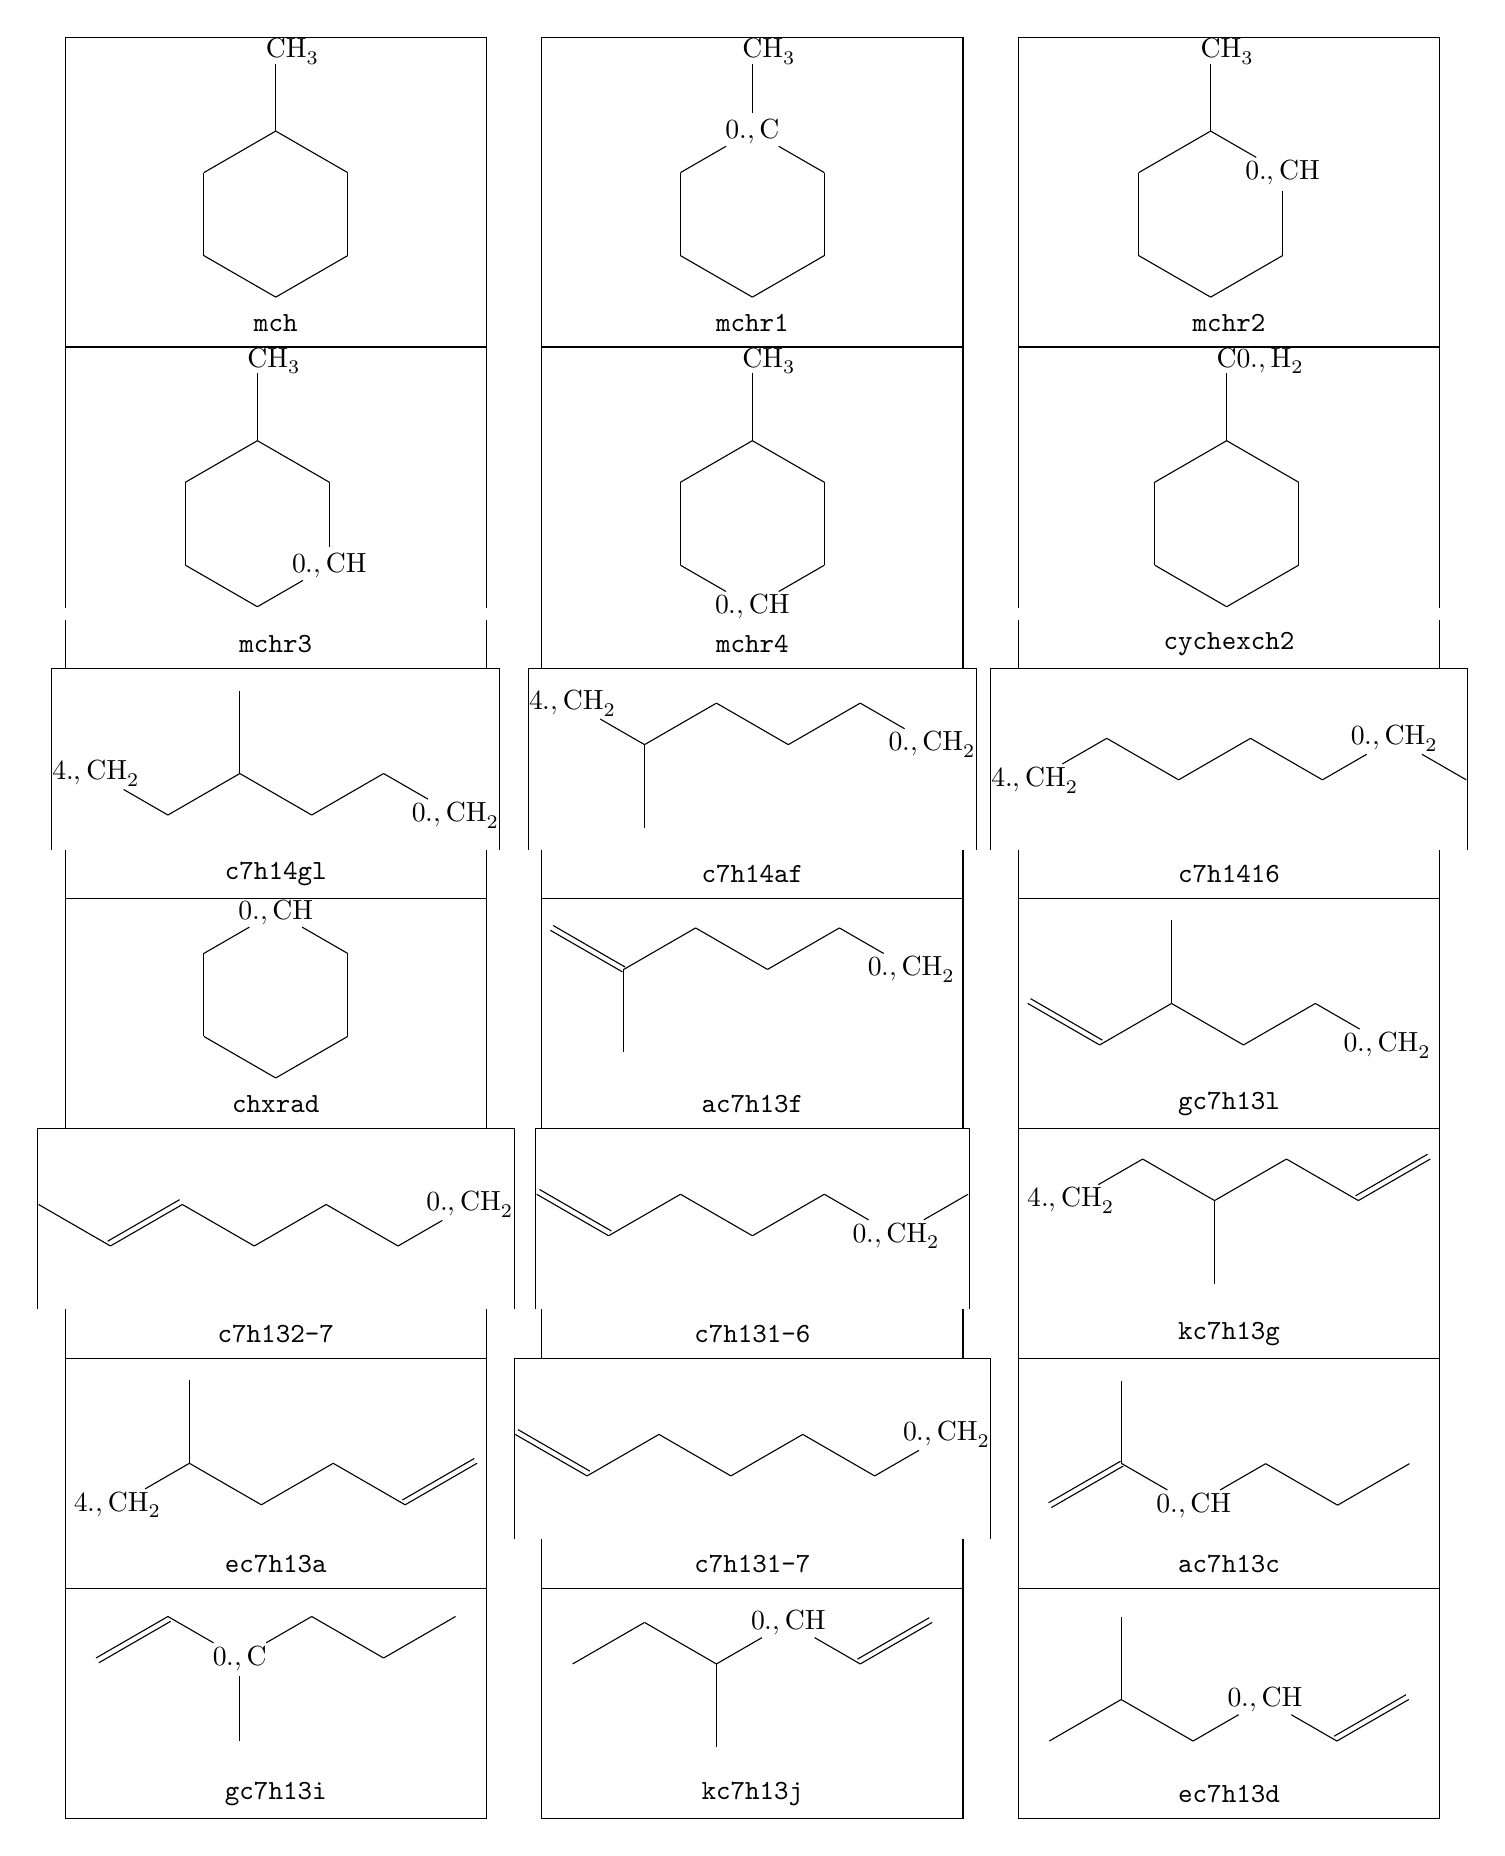
\begin{tikzpicture}
        \matrix[
            every odd row/.append style={nodes={top rectangle, inner sep=0pt, minimum height=0.9in}},
        ]
        {
            |[minimum height=1.25in]| \chemfig{CH_3-[6]*6(------)} &
            |[minimum height=1.25in]| \chemfig{CH_3-[6]\lewis{0.,C}*6(------)} &
            |[minimum height=1.25in]| \chemfig{CH_3-[6]*6(-----\lewis{0.,CH}-)} \\
            mch & mchr1 & mchr2 \\
            |[minimum height=1.25in]| \chemfig{CH_3-[6]*6(----\lewis{0.,CH}--)} &
            |[minimum height=1.25in]| \chemfig{CH_3-[6]*6(---\lewis{0.,CH}---)} &
            |[minimum height=1.25in]| \chemfig{{C}|\lewis{0.,H_2}-[6,,1]*6(------)} \\
            mchr3 & mchr4 & cychexch2 \\
            \chemfig{\lewis{4.,CH_2}-[:330]-[:30](-[2])-[:330]-[:30]-[:330]\lewis{0.,CH_2}} &
            \chemfig{\lewis{4.,CH_2}-[:330](-[6])-[:30]-[:330]-[:30]-[:330]\lewis{0.,CH_2}} &
            \chemfig{\lewis{4.,CH_2}-[:30]-[:330]-[:30]-[:330]-[:30]\lewis{0.,CH_2}-[:330]} \\
            c7h14gl & c7h14af & c7h1416 \\
            \chemfig{*6(----\lewis{0.,CH}--)} &
            \chemfig{=[:330](-[6])-[:30]-[:330]-[:30]-[:330]\lewis{0.,CH_2}} &
            \chemfig{=^[:330]-[:30](-[2])-[:330]-[:30]-[:330]\lewis{0.,CH_2}} \\
            chxrad & ac7h13f & gc7h13l \\
            \chemfig{-[:330]=^[:30]-[:330]-[:30]-[:330]-[:30]\lewis{0.,CH_2}} &
            \chemfig{=^[:330]-[:30]-[:330]-[:30]-[:330]\lewis{0.,CH_2}-[:30]} &
            \chemfig{\lewis{4.,CH_2}-[:30]-[:330](-[6])-[:30]-[:330]=^[:30]} \\
            c7h132-7 & c7h131-6 & kc7h13g \\
            \chemfig{\lewis{4.,CH_2}-[:30](-[2])-[:330]-[:30]-[:330]=^[:30]} &
            \chemfig{=^[:330]-[:30]-[:330]-[:30]-[:330]-[:30]\lewis{0.,CH_2}} &
            \chemfig{=[:30](-[2])-[:330]\lewis{0.,CH}-[:30]-[:330]-[:30]} \\
            ec7h13a & c7h131-7 & ac7h13c \\
            \chemfig{=_[:30]-[:330]\lewis{0.,C}(-[6])-[:30]-[:330]-[:30]} &
            \chemfig{-[:30]-[:330](-[6])-[:30]\lewis{0.,CH}-[:330]=^[:30]} &
            \chemfig{-[:30](-[2])-[:330]-[:30]\lewis{0.,CH}-[:330]=^[:30]} \\
            gc7h13i & kc7h13j & ec7h13d \\
        };
    \end{tikzpicture}
    \newpage
    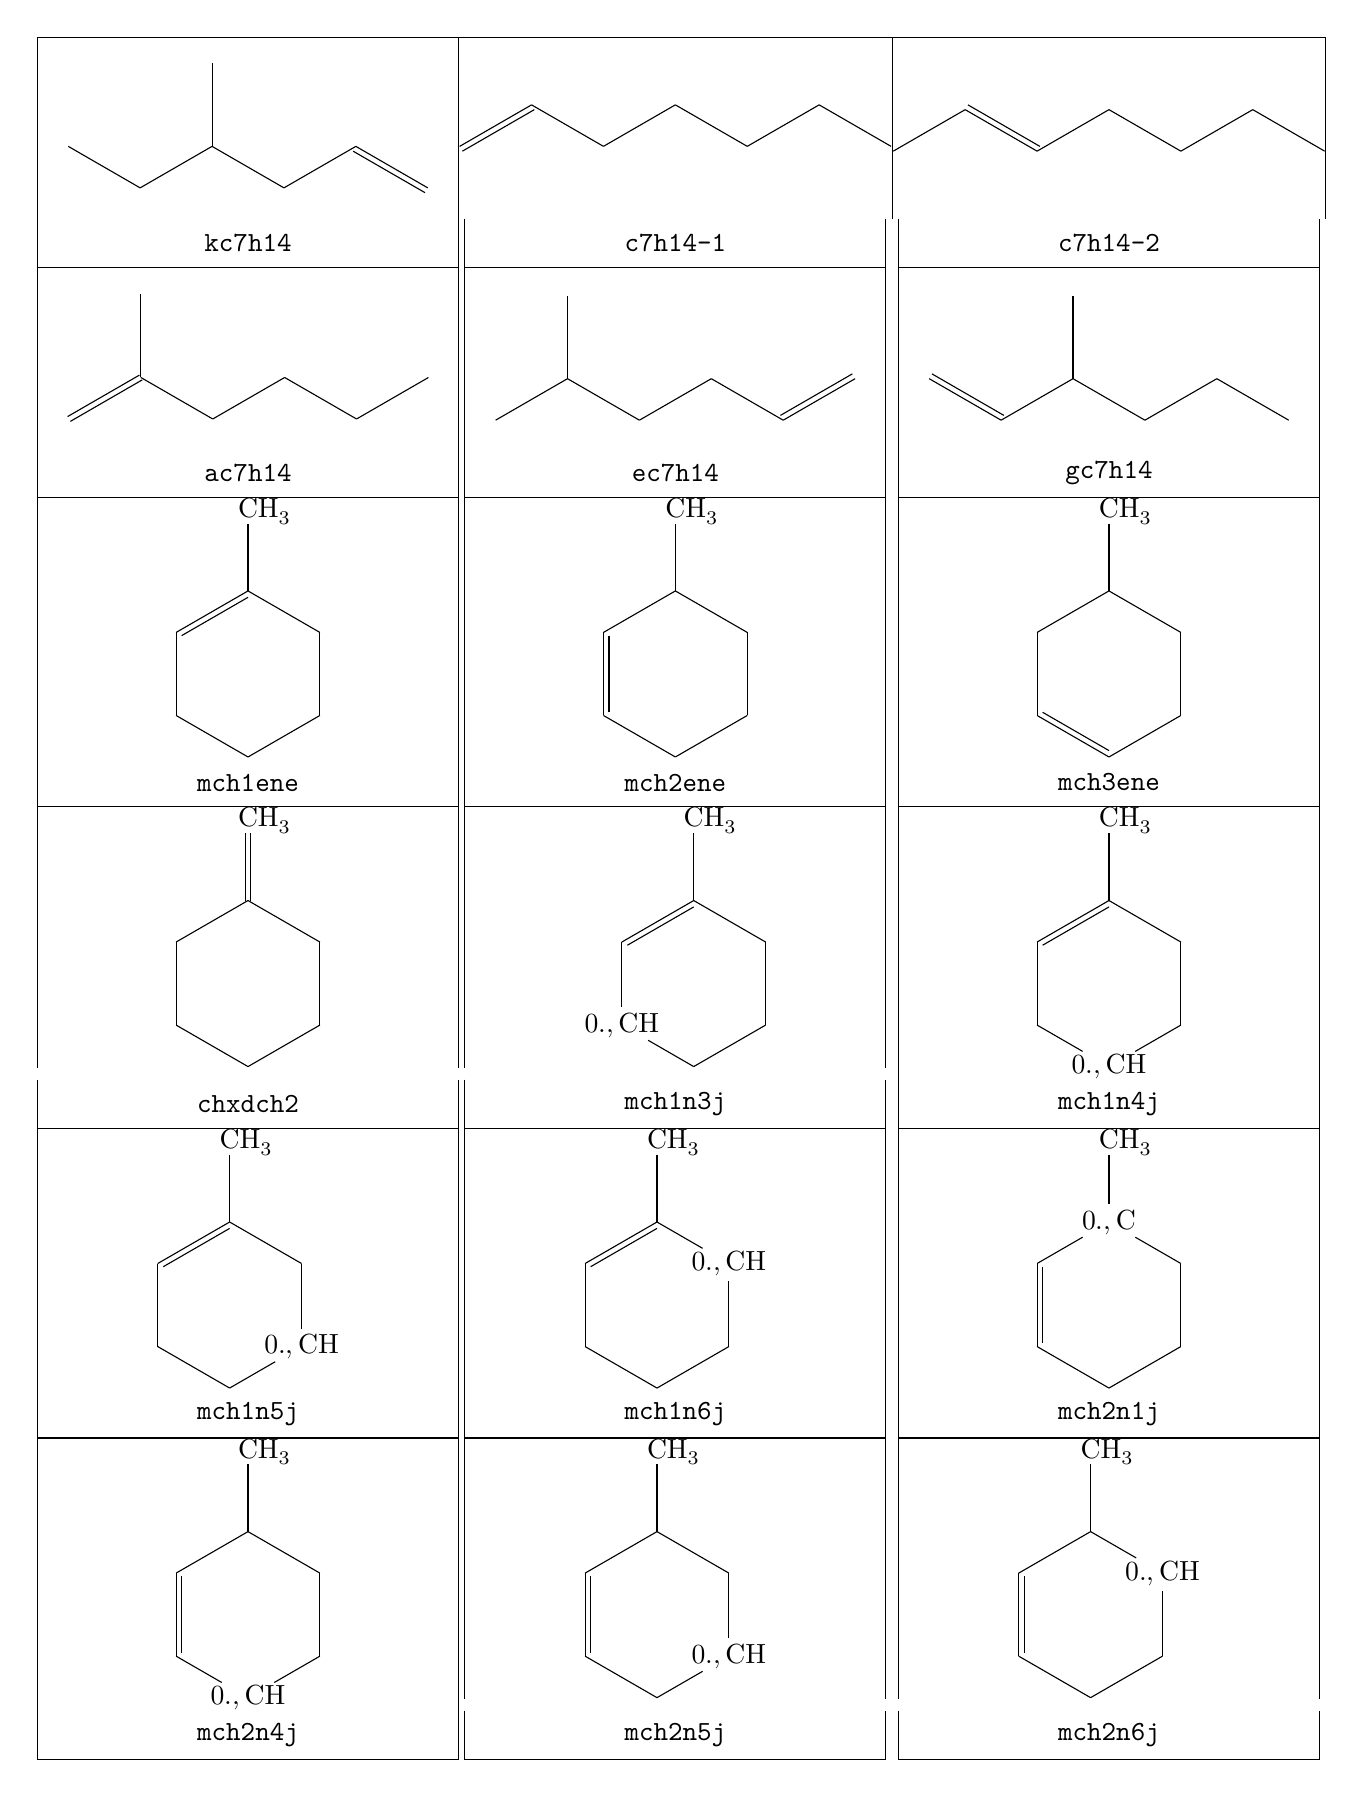
\begin{tikzpicture}
        \matrix[
            every odd row/.append style={nodes={top rectangle, inner sep=0pt, minimum height=1.25in}},
        ]
        {
            |[minimum height=0.9in]| \chemfig{-[:330]-[:30](-[2])-[:330]-[:30]=_[:330]} &
            |[minimum height=0.9in]| \chemfig{=_[:30]-[:330]-[:30]-[:330]-[:30]-[:330]} &
            |[minimum height=0.9in]| \chemfig{-[:30]=^[:330]-[:30]-[:330]-[:30]-[:330]} \\
            kc7h14 & c7h14-1 & c7h14-2 \\
            |[minimum height=0.9in]| \chemfig{=[:30](-[2])-[:330]-[:30]-[:330]-[:30]} &
            |[minimum height=0.9in]| \chemfig{-[:30](-[2])-[:330]-[:30]-[:330]=^[:30]} &
            |[minimum height=0.9in]| \chemfig{=^[:330]-[:30](-[2])-[:330]-[:30]-[:330]} \\
            ac7h14 & ec7h14 & gc7h14 \\
            \chemfig{CH_3-[6]*6(=-----)} &
            \chemfig{CH_3-[6]*6(-=----)} &
            \chemfig{CH_3-[6]*6(--=---)} \\
            mch1ene & mch2ene & mch3ene \\
            \chemfig{CH_3=[6]*6(------)} &
            \chemfig{CH_3-[6]*6(=-\lewis{0.,CH}----)} &
            \chemfig{CH_3-[6]*6(=--\lewis{0.,CH}---)} \\
            chxdch2 & mch1n3j & mch1n4j \\
            \chemfig{CH_3-[6]*6(=---\lewis{0.,CH}--)} &
            \chemfig{CH_3-[6]*6(=----\lewis{0.,CH}-)} &
            \chemfig{CH_3-[6]\lewis{0.,C}*6(-=----)} \\
            mch1n5j & mch1n6j & mch2n1j \\
            \chemfig{CH_3-[6]*6(-=-\lewis{0.,CH}---)} &
            \chemfig{CH_3-[6]*6(-=--\lewis{0.,CH}--)} &
            \chemfig{CH_3-[6]*6(-=---\lewis{0.,CH}-)} \\
            mch2n4j & mch2n5j & mch2n6j \\
        };
    \end{tikzpicture}
\end{center}
\end{document}